%%AMC:latex_engine=pdflatex --shell-escape
\documentclass[10pt,a4paper]{article}
\usepackage{needspace}
\usepackage[nobottomtitles]{titlesec}
\usepackage{multicol}
\usepackage{xcolor}
\usepackage{tikz}
\usepackage{circuitikz}
\usepackage{siunitx}
\usepackage{fp}
\usepackage{xfp}
\usepackage{WriteOnGrid}
\usepackage{csvsimple}%
\usepackage[francais,bloc]{automultiplechoice}

\FPseed=11

\baremeDefautS{e=0,v=0,b=1,m=-.25}
\baremeDefautM{e=0,v=0,b=.25,m=-.25}

\graphicspath{ {./images/} }


\newenvironment{reponsesd}{
    \begin{multicols}{2}
    \begin{reponses} }{
    \end{reponses}
    \end{multicols}
}

\setlength{\columnseprule}{1pt}
\def\columnseprulecolor{\color{lightgray}}%

\let\oexplain\explain
\renewcommand{\explain}[1]{\oexplain{\textcolor{red}{#1}}}


\titleformat{\section}
  {\centering\hrule\vspace{2mm}}
  {\thesection}
  {1em}
  {}
  [\vspace{1mm}\hrule]

\titleformat{\subsection}
  {\em}
  {\thesubsection}
  {1em}
  {}

\newcommand{\sujet}{
\exemplaire{1}{%

\AMCsetFoot{\niveau{}°\classe{} -- \prenom{}~\nom{} -- \thepage}

%%% debut de l'en-tête des copies :  
\begin{center}
\vfill
\noindent{\large \bf Classe de \niveau{}°\classe{}}

\vspace*{3mm}

{\Large\bf Évaluation sur table - Électricité 03/06/2024}

\vfill
\namefield{\noindent{}\fbox{\vspace*{3mm}
         \Huge\bf\prenom{}~\nom{}\normalsize{}% 
         \vspace*{3mm}
      }}
\end{center}
\vfill

\begin{center}
\textbf{Durée : 30 minutes.}
\vspace*{5mm}

  Aucun document n'est autorisé.
  L'usage de la calculatrice est interdit.

  Les questions faisant apparaitre le symbole \multiSymbole{} peuvent
  présenter une ou plusieurs bonnes réponses. Les autres ont
  une unique bonne réponse.

  Des points négatifs seront affectés aux mauvaises réponses.
  \vspace*{5mm}

  \textbf{IMPORTANT: Utilisez un crayon de papier pour cocher les cases, et une gomme pour effacer délicatement en cas d'erreur. Ne raturez pas les cases.}

  \vspace*{5mm}

  Ne pas faire comme ceci (pas centré, trop pâle, raturé):\\
  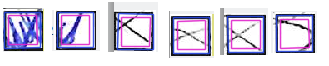
\includegraphics[width=4cm]{checkbox_bad.png}

  Mais comme cela (bien centré, bien foncé):\\
  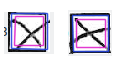
\includegraphics[width=2cm]{checkbox_good.png}


\end{center}
\vspace{1ex}
\vfill
\pagebreak
%%% fin de l'en-tête

\restituegroupe{groupes}


\AMCassociation{\id}

	  } % End \exemplaire{1}{%
} % End \newcommand{\sujet}{

%%%%§§§§§§§§§§§§§§§§§§§§§§§§§§§§§§§§§


\newcommand{\allq}{}

\begin{document}
%%%Options
\AMCrandomseed{11}

\def\AMCformQuestion#1{{\sc Question #1 :}}

\setdefaultgroupmode{withoutreplacement}
%%% Fin Options

%%% elements

\element{securite}{
  \begin{questionmult}{sec0}
    Pourquoi le courant électrique est dangereux pour les humains~?
    \FPeval\ySeed{trunc(random*1000,0) }
    \begin{reponsesd}
      \input{"|./genexo.py --seed \ySeed~ --mode S --level 0 --qref toto \allq"}
    \end{reponsesd}
  \end{questionmult}
}

\element{securite}{
  \begin{questionmult}{sec1}
    Quelles sources de courants sont dangereuses pour les humains~?
    \FPeval\ySeed{trunc(random*1000,0) }
    \begin{reponsesd}
      \input{"|./genexo.py --seed \ySeed~ --mode S --level 1 --qref toto \allq"}
    \end{reponsesd}
  \end{questionmult}
}

\element{securite}{
  \begin{questionmult}{sec2}
    Cochez les situation ou l'électrocution est un risque avéré~:
    \FPeval\ySeed{trunc(random*1000,0) }
    \begin{reponsesd}
      \input{"|./genexo.py --seed \ySeed~ --mode S --level 2 --qref toto \allq"}
      \bonne{Démonter un micro-onde débranché}\bareme{m=0}
    \end{reponsesd}
    \explain{Certains appareils électriques, comme les micro-ondes comportent des condensateurs haute-tension qui peuvent rester chargés après débranchement de l'appareil.}
   \end{questionmult}
}


\FPeval\ySeed{trunc(random*1000,0)}
\input{"|./genexo.py --seed \ySeed~ --mode SYM --level 0 --qref toto \allq"}


\element{symboles}{
  \begin{question}{sym4}
    Quel interrupteur est fermé~?

    \begin{reponses}
      \mauvaise{\includegraphics[width=2cm]{ouvert.png}}
      \bonne{\includegraphics[width=2cm]{ferme.png}}
      \mauvaise{\includegraphics[width=2cm]{lamp.png}}
      \mauvaise{\includegraphics[width=2cm]{generator.png}}
    \end{reponses}
    \explain{Un interrupteur fermé laisse passer le courant: c'est donc celui qui connecte ses deux bornes.}
  \end{question}
}

\element{symboles}{
  \begin{question}{sym5}
    Un interrupteur~:

    \begin{reponses}
      \mauvaise{Laisse passer le courant lorsqu'il est ouvert}
      \bonne{Laisse passer le courant Lorsqu'il est fermé}
      \mauvaise{Laisse toujours passer le courant}
      \mauvaise{Ne laisse jamais passer le courant}
    \end{reponses}
  \end{question}
}

\element{seriederiv}{
  \begin{question}{sdv1}
  \needspace{6cm}
    Ce montage est-il en série ou en dérivation~?
    \begin{circuitikz}[european]
      \draw (0,0)
      to [ american voltage source, invert, o-o] (0,3);
      \draw (0,0)
      to [ lamp, o-o]  (4,0);
      \draw (4,0)
      to [ lamp, o-o]  (4,3);
      \draw (4,3)
      to [ lamp, o-o]  (0,3);
	\end{circuitikz}    
    \begin{reponses}
      \bonne{Le montage est branché en série}
      \mauvaise{Le montage est branché en dérivation}
    \end{reponses}
  \end{question}
}

\element{seriederiv}{
  \begin{question}{sdv2}
  \needspace{6cm}
    Ce montage est-il en série ou en dérivation~?

	\begin{circuitikz}[european]
	 \draw (0,0) -- (4,0);
	 \draw (0,3) -- (4,3);
	
	 \draw (0,0)
	 to [ american voltage source, invert, o-o] (0,3);
	 \draw (2,0)
	 to [ lamp, o-o]  (2,3);
	 \draw (4,0)
	 to [ lamp, o-o]  (4,3);
	\end{circuitikz}    
    
    \begin{reponses}
      \mauvaise{Le montage est branché en série}
      \bonne{Le montage est branché en dérivation}
    \end{reponses}
  \end{question}
}

\element{mesures}{
  \begin{question}{mes1}
    Comment appelle t'on cet appareil~?
    \\
    \includegraphics[angle=90,origin=c,height=3cm]{multimetre.jpg}
    \vspace*{-1cm}
    \begin{reponsesd}
      \mauvaise{Un manomètre}
      \bonne{Un multimètre}
      \mauvaise{Un électromètre}
      \mauvaise{Un Grand Maitre}
    \end{reponsesd}
    \explain{Il est appelé multimètre parce qu'il comporte plusieurs (multi fonctions) ampèremètre, voltmètre, ohmmètre, etc.}
  \end{question}
}

\element{mesures2}{
  \begin{question}{mes2}
    Sur quelle zone faut-il régler l'appareil pour mesurer l'intensité d'un courant électrique~?
    \begin{reponsesd}
      \mauvaise{\includegraphics[height=2cm]{multimetreV.jpg}}
      \bonne{\includegraphics[height=2cm]{multimetreA.jpg}}
      \mauvaise{\includegraphics[height=2cm]{multimetreO.jpg}}
      \mauvaise{\includegraphics[height=2cm]{multimetreZ.jpg}}
    \end{reponsesd}
  \end{question}
}

\element{mesures2}{
  \begin{question}{mes3}
    Sur quelle zone faut-il régler l'appareil pour mesurer la tension électrique entre deux points~?
    \begin{reponsesd}
      \mauvaise{\includegraphics[height=2cm]{multimetreA.jpg}}
      \bonne{\includegraphics[height=2cm]{multimetreV.jpg}}
      \mauvaise{\includegraphics[height=2cm]{multimetreO.jpg}}
      \mauvaise{\includegraphics[height=2cm]{multimetreZ.jpg}}
    \end{reponsesd}
  \end{question}
}

\element{mesures}{
  \begin{question}{mes4}
    Lorsque l'on veut faire une mesure sur une tension ou intensité que l'on ne connait pas, sur quel calibre met-on l'appareil~?
    \begin{reponsesd}
      \bonne{On commence par le calibre le plus élevé}
      \mauvaise{On commence par le calibre le plus petit}
      \mauvaise{Peu importe}
      \mauvaise{On place la fiche sur le calibre \qty{10}{\A}}
   \end{reponsesd}
   \explain{On commence toujours par le calibre le plus grand pour éviter d'endomager l'appareil de mesure. Toutefois, le calibre \qty{10}{\A} n'étant pas protégé par un fusible, nous ne l'utilisons pas.}
  \end{question}
}

\element{mesures}{
  \begin{question}{mes5}
    L'appareil affiche cet écran lors d'une mesure en voltmètre, alors~:
    \\
    \includegraphics[width=4cm]{multimetreover.jpg}
    \begin{reponsesd}
      \bonne{La valeur est trop élevée, il faut passer au calibre supérieur}
      \mauvaise{\clubpenalties 1 10000 La valeur est trop basse, il faut passer au calibre inférieur}
      \mauvaise{La valeur mesurée est de 1V exactement}
      \mauvaise{L'appareil n'est pas branché}
    \end{reponsesd}
    \explain{Le multimètre indique ici que la valeur est trop élevée pour être affichée. Il faut donc passer sur un calibre plus élevé àfin de faire la mesure.}
  \end{question}
}

\element{mesures3}{
  \begin{questionmult}{mes6}
    Vous souhaitez mesurer le courant qui passe dans l'élément $L_1$, comment branchez vous l'ampèremètre~?
    \begin{reponsesd}
      \bonne{
        \begin{circuitikz}[european,scale = 0.7]
          \draw (0,0) to [ rmeter, t=A ] (4,0);
          \draw (0,3) -- (4,3);
          \draw (0,3) to [ rmeter, t=G,v=\empty, american voltages ] (0,0);
          \draw (4,0) to [ lamp=$L_1$, o-o]  (4,3);
        \end{circuitikz}
      }
      \bonne{
        \begin{circuitikz}[european,scale = 0.7]
          \draw (0,3) to [ rmeter, t=A ] (4,3);
          \draw (0,0) -- (4,0);
          \draw (0,3) to [ rmeter, t=G,v=\empty, american voltages ] (0,0);
          \draw (4,0) to [ lamp=$L_1$, o-o]  (4,3);
        \end{circuitikz}
      }
      \mauvaise{
        \begin{circuitikz}[european,scale = 0.7]
          \draw (0,0) -- (4,0);
          \draw (0,3) -- (4,3);
          \draw (0,3) to [ rmeter, t=G,v=\empty, american voltages ] (0,0);
          \draw (2,0) to [ rmeter, t=A ]  (2,3);
          \draw (4,0) to [ lamp=$L_1$, o-o]  (4,3);
        \end{circuitikz}
      }
      \mauvaise{
        \begin{circuitikz}[european,scale = 0.7]
          \draw (0,0) -- (4,0);
          \draw (0,3) -- (4,3);
          \draw (0,3) to [ rmeter, t=G,v=\empty, american voltages ] (0,0);
          \draw (4,0) to [ rmeter, t=A ]  (4,3);
          \draw (2,0) to [ lamp=$L_1$, o-o]  (2,3);
        \end{circuitikz}
      }
    \end{reponsesd}
    \explain{Un ampèremètre se place toujours en série sur le circuit, il mesure l'intensité qui le traverse. Branché en dérivation, il provoque un cours-circuit.}
  \end{questionmult}
}

\element{mesures3}{
  \begin{questionmult}{mes7}
    Vous souhaitez mesurer la tension aux bornes de l'élément $L_1$, comment branchez vous le voltmètre~?
    \begin{reponsesd}
      \mauvaise{
        \begin{circuitikz}[european,scale = 0.7]
          \draw (0,0) to [ rmeter, t=V ] (4,0);
          \draw (0,3) -- (4,3);
          \draw (0,3) to [ rmeter, t=G,v=\empty, american voltages ] (0,0);
          \draw (4,0) to [ lamp=$L_1$, o-o]  (4,3);
        \end{circuitikz}
      }
      \mauvaise{
        \begin{circuitikz}[european,scale = 0.7]
          \draw (0,3) to [ rmeter, t=V ] (4,3);
          \draw (0,0) -- (4,0);
          \draw (0,3) to [ rmeter, t=G,v=\empty, american voltages ] (0,0);
          \draw (4,0) to [ lamp=$L_1$, o-o]  (4,3);
        \end{circuitikz}
      }
      \bonne{
        \begin{circuitikz}[european,scale = 0.7]
          \draw (0,0) -- (4,0);
          \draw (0,3) -- (4,3);
          \draw (0,3) to [ rmeter, t=G,v=\empty, american voltages ] (0,0);
          \draw (2,0) to [ rmeter, t=V ]  (2,3);
          \draw (4,0) to [ lamp=$L_1$, o-o]  (4,3);
        \end{circuitikz}
      }
      \bonne{
        \begin{circuitikz}[european,scale = 0.7]
          \draw (0,0) -- (4,0);
          \draw (0,3) -- (4,3);
          \draw (0,3) to [ rmeter, t=G,v=\empty, american voltages ] (0,0);
          \draw (4,0) to [ rmeter, t=V ]  (4,3);
          \draw (2,0) to [ lamp=$L_1$, o-o]  (2,3);
        \end{circuitikz}
      }
    \end{reponsesd}
    \explain{Un voltmètre se place toujours en dérivation sur le dipole à mesurer, car il prend la différence de potentiel entre ses bornes. Placé en série, il se comporte comme un interrupteur oiuvert et bloque le courant.}
  \end{questionmult}
}

\element{introcalculs1}{
  \begin{questionmult}{ical1}
    Dans un circuit électrique monté en série, on peut appliquer ~:
    \begin{reponsesd}
      \bonne{La loi d'unicité de l'intensité du courant électrique}
      \bonne{La loi d’additivité des tensions électrique}
      \mauvaise{La loi d’additivité des intensités du courant électrique}
      \mauvaise{La loi d'unicité des tensions électriques}
    \end{reponsesd}
  \end{questionmult}
}

\element{introcalculs1}{
  \begin{questionmult}{ical2}
    Dans un circuit électrique monté en dérivation, on peut appliquer~:
    \begin{reponsesd}
      \bonne{La loi d'unicité des tensions électriques}
      \bonne{La loi d’additivité des intensités du courant électrique}
      \mauvaise{La loi d’additivité des tensions électrique }
      \mauvaise{La loi d'unicité de l'intensité du courant électrique}
    \end{reponsesd}
  \end{questionmult}
}


\element{introcalculs2}{
  \begin{question}{ical3}
    Cochez la case où l'égalité est respectée~:
    \begin{reponsesd}
      \bonne   {\qty{1}{\A}=\qty{1000}{\mA}}
      \mauvaise{\qty{1}{\A}=\qty{100}{\mA}}
      \mauvaise{\qty{1}{\A}=\qty{10}{\mA}}
      \mauvaise{\qty{1}{\A}=\qty{1}{\mA}}
    \end{reponsesd}
   \explain{En unité SI, le préfixe 'm' signifie 'mili' et veut dire $1/1000$ ou $0.001$, aussi $\qty{1}{\A}=\qty{1000}{\mA}$ }
  \end{question}
}
\element{introcalculs2}{
  \begin{question}{ical4}
    Cochez la case où l'égalité est respectée~:
    \begin{reponsesd}
      \bonne   {\qty{1}{\V}=\qty{1000}{\mV}}
      \mauvaise{\qty{1}{\V}=\qty{100}{\mV}}
      \mauvaise{\qty{1}{\V}=\qty{10}{\mV}}
      \mauvaise{\qty{1}{\V}=\qty{1}{\mV}}
    \end{reponsesd}
    \explain{En unité SI, le préfixe 'm' signifie 'mili' et veut dire $1/1000$ ou $0.001$, aussi $\qty{1}{\V}=\qty{1000}{\mV}$ }
  \end{question}
}

\element{introcalculs}{
  \begin{questionmult}{ical5}
    Cochez les case où l'égalité est respectée~:
    \FPeval\ySeed{trunc(random*1000,0) }
    \input{"|./genexo.py --seed \ySeed~ --mode C --level 0 --qref toto"}
  \end{questionmult}
}

\element{calculs1}{
  \FPeval\ySeed{trunc(random*1000,0) }
  \input{"|./genexo.py --seed \ySeed~ --mode A --level 0 --qref cal11"}
}

\element{calculs1}{
  \FPeval\ySeed{trunc(random*1000,0) }
  \input{"|./genexo.py --seed \ySeed~ --mode A --level 1 --qref cal12"}
}

\element{calculs2}{
  \FPeval\ySeed{trunc(random*1000,0) }
  \input{"|./genexo.py --seed \ySeed~ --mode A --level 2 --qref cal21"}
}

\element{calculs2}{
  \FPeval\ySeed{trunc(random*1000,0) }
  \input{"|./genexo.py --seed \ySeed~ --mode A --level 2 --qref cal22"}
}

\element{calculs3}{
  \FPeval\ySeed{trunc(random*1000,0) }
  \input{"|./genexo.py --seed \ySeed~ --mode A --level 3 --qref cal31"}
}

\element{calculs3}{
  \FPeval\ySeed{trunc(random*1000,0) }
  \input{"|./genexo.py --seed \ySeed~ --mode A --level 3 --qref cal32"}
}

\element{calculs4}{
  \FPeval\ySeed{trunc(random*1000,0) }
  \input{"|./genexo.py --seed \ySeed~ --mode A --level 4 --qref cal41"}
}

\element{calculs4}{
  \FPeval\ySeed{trunc(random*1000,0) }
  \input{"|./genexo.py --seed \ySeed~ --mode A --level 4 --qref cal42"}
}

\element{calculs1}{
  \FPeval\ySeed{trunc(random*1000,0) }
  \input{"|./genexo.py --seed \ySeed~ --mode V --level 0 --qref calv1"}
}

\element{calculs2}{
  \FPeval\ySeed{trunc(random*1000,0) }
  \input{"|./genexo.py --seed \ySeed~ --mode V --level 1 --qref calv2"}
}

\element{calculs1}{
  \FPeval\ySeed{trunc(random*1000,0) }
  \input{"|./genexo.py --seed \ySeed~ --mode V --level 0 --qref calv3"}
}

\element{calculs2}{
  \FPeval\ySeed{trunc(random*1000,0) }
  \input{"|./genexo.py --seed \ySeed~ --mode V --level 1 --qref calv4"}
}


\element{groupes}{
\section{Sécurité}
%\begin{multicols}{2}
\restituegroupe[2]{securite}
%\end{multicols}

\section{La représentation des circuits électriques}
\begin{multicols}{2}
\restituegroupe[3]{autosymboles}
\restituegroupe[1]{symboles}
\end{multicols}

\section{Mesures de courants et de tensions dans les circuits électriques}
%\begin{multicols}{2}
\restituegroupe{mesures}
\restituegroupe[1]{mesures2}
\restituegroupe[1]{mesures3}
%\end{multicols}

\section{Types de circuits électriques}
\begin{multicols}{2}
\restituegroupe{seriederiv}
\end{multicols}

\section{Notions d'intensité et de tension électrique}
\restituegroupe[1]{introcalculs1}
\restituegroupe[1]{introcalculs2}
\restituegroupe{introcalculs}

\needspace{8cm}
\section{Calculs d'intensités du courant électrique}
\begin{multicols}{2}
\restituegroupe[2]{calculs1}
\restituegroupe[2]{calculs2}
\restituegroupe[2]{calculs3}
\restituegroupe[2]{calculs4}
\end{multicols}

\section{Petit problème}

\emph{Ce problème est plus difficile et rapporte moins de points, ne le faire que lorsque le reste est terminé, c'est un bonus!}

Soit le circuit suivant. Toutes les lampes du circuit sont identiques. L’ampèremètre affiche $I=\qty{0,90}{\A}$ et le générateur a une tension de $U=\qty{9} {\V}$.

 \begin{circuitikz}[european,scale = 0.7]
          \draw ( 0,0) to [ lamp=$L_5$, o-o ] (0,4);
          \draw ( 3,0) to [ lamp=$L_6$, o-o ] (3,4);
          \draw ( 3,0) to [ lamp=$L_4$, o-o ] (9,0);
          \draw ( 3,4) to [ rmeter, t=A ]  (6,4);
          \draw ( 6,4) to [ rmeter, t=G,v=$\qty{9}{\V}$, american voltages ] (9,4);
          \draw ( 9,0) to [ lamp=$L_1$, o-o ] ( 9,4);
          \draw (12,0) to [ lamp=$L_2$, o-o ] (12,4);
          \draw (15,0) to [ lamp=$L_3$, o-o ] (15,4);
          \draw (0,0) -- ( 3,0);
          \draw (0,4) -- ( 3,4);
          \draw (9,0) -- (15,0);
          \draw (9,4) -- (15,4);
       \end{circuitikz}
\subsection{Redessine le schéma électrique pour qu’il soit plus compréhensible}

\begin{EnvQuadrillage}[NbCarreaux=30x12,Grille=5x5]
\end{EnvQuadrillage}

\subsection{Quelle est l’intensité qui traverse chacune des lampes~? (Justifiez)}

\begin{EnvQuadrillage}[NbCarreaux=21x8,Grille=Seyes,Marge=1]
\end{EnvQuadrillage}

\subsection{Quelles lampes ont le même éclairement~?}

\begin{EnvQuadrillage}[NbCarreaux=21x2,Grille=Seyes,Marge=1]
\end{EnvQuadrillage}

\subsection{Quelle lampe brille le plus~?}

\begin{EnvQuadrillage}[NbCarreaux=21x2,Grille=Seyes,Marge=1]
\end{EnvQuadrillage}

\subsection{Indiquez sur le schéma que vous avez redessiné, par des flèches, le sens du courant dans chaque lampe.}

\AMCcleardoublepage
}


\csvreader[head to column names]{liste.csv}{}{\sujet}

\end{document}


